% Faithful Strategy Explanations Grounded in F1 Telemetry
% Official ACL template (acl.sty). Use [review] for anonymous submission;
% kept non-review here to show the author as requested.
\documentclass[11pt]{article}
\usepackage[]{acl}
\usepackage{times}
\usepackage{latexsym}
\usepackage{booktabs}
\usepackage{graphicx}
\usepackage{xcolor}
\usepackage{amssymb}
\usepackage[T1]{fontenc}
\usepackage[utf8]{inputenc}
\usepackage{microtype}

\newcommand{\FOneNumRaces}{157}
\newcommand{\FOneNumInstances}{7253}
\newcommand{\FOneNumSeasons}{8}
\newcommand{\FOneFirstSeason}{2018}
\newcommand{\FOneLastSeason}{2026}
\newcommand{\FOneNumTrain}{6004}
\newcommand{\FOneNumTest}{1249}
\newcommand{\FOneNumTestSample}{207}
\newcommand{\FOneNumStint}{1500}
\newcommand{\FOneNumUndercut}{2034}
\newcommand{\FOneNumOvercut}{1125}
\newcommand{\FOneNumDefense}{2444}
\newcommand{\FOneNumRaceSummary}{150}
\newcommand{\FOneNumStints}{8486}
\newcommand{\FOneNumPits}{5358}
\newcommand{\FOneNumBattles}{3337}

\IfFileExists{result_macros.tex}{\newcommand{\JudgePearson}{0.55}
\newcommand{\JudgeSpearman}{0.54}
\newcommand{\JudgeN}{120}
\newcommand{\JudgeModel}{gpt-5.5}
\newcommand{\MethodFirst}{0.640}
\newcommand{\MethodFinal}{0.881}
\newcommand{\MethodModel}{gpt-5.4-mini}
\newcommand{\MethodErrors}{0}
\newcommand{\ExtractorEnSpearman}{0.80}
\newcommand{\ExtractorEnPearson}{0.50}
\newcommand{\ExtractorEnN}{564}
\newcommand{\ExtractorInstPearson}{0.49}
\newcommand{\ExtractorN}{1527}
\newcommand{\XfamSpearman}{1.00}
\newcommand{\XfamPearson}{0.82}
\newcommand{\XfamN}{1090}
\newcommand{\XfamModel}{DeepSeek-V3.2}
\newcommand{\CovLang}{PT}
\newcommand{\CovFlipModel}{grok-4.3}
\newcommand{\CovFlipPrec}{0.89}
\newcommand{\CovFlipRecall}{0.46}
\newcommand{\CovFlipFone}{0.61}
\newcommand{\CovFlipFRank}{last}
\newcommand{\CovTopFoneModel}{claude-sonnet-4-6}
\newcommand{\CovTopFone}{0.83}
\newcommand{\CovRankChanges}{yes}
\newcommand{\WxGeminiPrec}{0.91}
\newcommand{\WxGeminiRecall}{0.48}
\newcommand{\WxGeminiClaims}{3.0}
\newcommand{\WxOthersRecall}{0.50--0.85}
\newcommand{\WxFlip}{yes}
\newcommand{\AblMeanRecallA}{0.60}
\newcommand{\AblMeanRecallB}{0.47}
\newcommand{\AblNModels}{5}
\newcommand{\AblNUp}{2}
\newcommand{\RSLoPrecModel}{DeepSeek-V3.2}
\newcommand{\RSLoPrec}{0.49}
\newcommand{\RSLoRecall}{0.42}
\newcommand{\RSDeepseekPrec}{0.49}
\newcommand{\RSDeepseekRecall}{0.42}
}{}

\title{Precision Is Not Faithfulness: Coverage-Aware Evaluation of\\
Grounded Generation with a Complete Oracle}
\author{Juan S. Santillana\thanks{The author is a DevOps Engineer at Globant;
  academic affiliation pending.} \\
  \texttt{juan.salas@globant.com}}

\begin{document}
\maketitle

\begin{abstract}
Reference-free faithfulness metrics verify each atomic claim a model makes against
ground truth, and are increasingly used to evaluate grounded generation. We show they
share a blind spot: they measure only \emph{precision} -- are the stated claims
supported? -- and therefore \emph{reward abstention}, since a model can score
near-perfect faithfulness by saying almost nothing. We make this measurable using
Formula~1 telemetry, a domain where strategic ground truth is derived deterministically
and, crucially, \emph{completely}: for each decision we know the full set of facts that
mattered. This completeness -- absent in open-domain faithfulness benchmarks -- lets us
measure \emph{recall} (coverage of the relevant facts) alongside precision. On a
multilingual (EN/ES/PT) benchmark of \FOneNumInstances{} decision instances spanning
\FOneNumRaces{} races, the most ``faithful'' frontier model attains precision
\CovGeminiPrec{} yet covers only \CovGeminiRecall{} of the relevant facts, and requiring
coverage \emph{inverts the model ranking}, moving it from first to last; the same
abstention behavior reappears in a second complete-oracle domain (weather forecasts). We
pair faithfulness with coverage into a single score, validate the metric (controlled
perturbation; agreement across a model-free regex extractor and a cross-family LLM
extractor, system-level Spearman \XfamSpearman{}), and give a verifier-guided generation
method that improves precision and recall without references. We release the benchmark,
structured annotations, metric, baselines, and an interactive demo.
\end{abstract}

\section{Introduction}
Reference-free faithfulness metrics -- which decompose a generation into atomic claims
and verify each against ground truth
\citep{min2023factscore,fabbri2022qafacteval} -- have become a standard way to evaluate
grounded generation without gold reference texts. They report a \emph{precision}: of the
claims the model made, how many are supported? We argue this is only half of what
``faithful'' should mean. A model can maximize precision by being maximally cautious --
stating one safe fact and omitting everything else. A precision-only metric scores such
output as near-perfect, even though it is uninformative. Faithfulness, measured as
precision alone, \emph{rewards abstention}.

The missing half is \emph{recall}: of the facts that mattered, how many did the model
correctly state? Open-domain faithfulness benchmarks cannot measure this, because there
is no complete, enumerable set of relevant facts to recall against -- the ground truth
is whatever a retriever or annotator happened to surface. We therefore turn to a domain
with a \emph{complete} oracle. Formula~1 produces rich, public timing and telemetry data
from which strategic ground truth (pit laps, compounds, undercuts, defenses, outcomes)
can be derived \emph{deterministically and exhaustively}: for each decision we know the
full set of checkable facts. This lets us measure recall, and pair it with precision,
in a way open-domain settings structurally cannot.

Using this oracle we show the abstention problem is not hypothetical: on a multilingual
benchmark, the frontier model with the highest faithfulness (precision) covers only
\CovGeminiRecall{} of the relevant facts, and once coverage is required the model ranking
\emph{inverts} (Section~\ref{sec:exp}). We frame F1 strategy explanation as faithful,
data-grounded NLG -- not race-outcome prediction, which is saturated and outside language
research -- because it gives the cleanest available testbed for this measurement question.

\noindent Our contributions:
\begin{enumerate}
  \item We show that reference-free faithfulness metrics reward abstention, and that with
        a \emph{complete} oracle the model ranking inverts when coverage is required --
        replicated across two unrelated domains, F1 and weather
        (Section~\ref{sec:exp}, \ref{sec:weather}).
  \item A complete-oracle, multilingual (EN/ES/PT) benchmark of \FOneNumInstances{}
        grounded F1 decision instances, and a precision+recall faithfulness metric,
        validated by controlled perturbation and by agreement across a model-free and a
        cross-family extractor (Section~\ref{sec:data}, \ref{sec:metric}).
  \item A verifier-guided generation method that improves both precision and recall using
        only the structured verifier as signal (Section~\ref{sec:method}).
\end{enumerate}
\noindent The benchmark, metric, baselines, and an interactive demo are
public.\footnote{Demo: \url{https://huggingface.co/spaces/jsantillana/faithful-strategy-engineer-f1}}

\section{Related Work}
Data-to-text generation has a long line of sports work, e.g. RotoWire
\citep{wiseman2017challenges} and SportSett:Basketball
\citep{thomson2020sportsett}, and controlled table-to-text such as ToTTo
\citep{parikh2020totto}. Faithfulness/hallucination evaluation includes FActScore
\citep{min2023factscore}, QA-based consistency \citep{fabbri2022qafacteval}, and
NLI-based inconsistency detection \citep{laban2022summac,kryscinski2020factcc};
see \citet{ji2023survey} for a survey. These reference-free metrics are
precision-oriented: they score the claims a model makes, not the ones it omits, and so
do not penalize an uninformative output -- the abstention blind spot we study. The
complementary, recall side has been recognized in table-to-text via PARENT
\citep{dhingra2019parent}, which credits coverage of the source table, but it requires a
reference text and a (possibly incomplete) table; our oracle is reference-free and
complete, letting us measure recall directly against the full fact set. Our
verifier-guided generation relates to self-refinement with feedback
\citep{madaan2023selfrefine}, but the feedback signal here is a deterministic check
against structured data rather than the model's own critique. Unlike reference-based
sports NLG, we evaluate both faithfulness and coverage directly against structured data
(reference-free) and add a multilingual axis. Our use of a compact, domain-specialized
model follows recent work on small efficient models with native tool use for Spanish
technical domains \citep{vectrayxnano2026}.

\section{Task}\label{sec:task}
Each instance provides a structured context (driver stints, tyre compound and
age, pit stops, gaps, safety-car/VSC status) and a decision prompt in EN/ES/PT.
The model must explain a strategic decision such that every factual claim is
verifiable against the context. The benchmark spans five decision types: tyre
strategy, undercut, overcut, \emph{on-track defense} (a faster pursuer kept behind
for several laps -- the ``rear gunner'' move), and \emph{race summary} (a grounded
recap of result and key moments).

\section{Dataset}\label{sec:data}
We extract timing and telemetry with FastF1 \citep{fastf1} (the official live-timing
API; no broadcast access required) and derive strategic events with deterministic
rules. Stints are segmented per driver with a within-stint degradation slope fit on
\emph{green-flag} laps only (excluding in/out laps and laps under yellow, safety car
(SC), or virtual safety car (VSC)) so that pace estimates are not contaminated by
neutralizations. Pit stops are recovered from stint transitions and flagged when made
under SC/VSC. Undercuts and overcuts are detected pairwise but kept only for drivers
genuinely racing each other -- within a small on-track gap so the pit sequence, not
accumulated pace difference, dominates the gap swing -- which yields high-precision
events (spot-checked against known race narratives, e.g.\ the winning one-stop at the
2024 Italian GP). On-track defenses are detected as runs of $\geq 5$ consecutive laps
in which a pace-faster pursuer is held within $1.5$s, flagged when a teammate is
protected ahead; this recovers canonical cases (e.g.\ Alonso holding Hamilton for
$11$ laps, Hungary 2021). Season standings (race plus sprint points) support grounded
championship summaries.

Each instance pairs a serialized structured context with a decision prompt in EN/ES/PT
and the structured ground truth used for verification. From \FOneNumRaces{} races
across \FOneNumSeasons{} seasons (\FOneFirstSeason{}--\FOneLastSeason{}) we obtain
\FOneNumStints{} stints, \FOneNumPits{} pit stops, and \FOneNumBattles{} pit battles,
yielding \FOneNumInstances{} instances (\FOneNumStint{} tyre-strategy,
\FOneNumUndercut{} undercut, \FOneNumOvercut{} overcut, \FOneNumDefense{} defense,
\FOneNumRaceSummary{} race-summary). To avoid leakage we split by
season: \FOneNumTrain{} train instances (\FOneFirstSeason{}--2024) and \FOneNumTest{}
held-out test instances (\FOneLastSeason{}); the model comparisons below use a
stratified test sample of \FOneNumTestSample{} instances. We do not redistribute raw
FOM data; we release the derived structured ground truth, annotations, and code
(Section~\ref{sec:ethics}).

\paragraph{A complete oracle.} The key property we exploit is that this ground truth is
not just deterministic but \emph{complete}: for each decision instance we can enumerate
the full set of checkable facts that a good explanation should cover -- for a stint, the
driver's stop count, pit laps, compound changes, and finishing position; for an
undercut/overcut, the two pit laps, the move and its outcome, and the time gained. This
enumerable fact set is the denominator for recall (Section~\ref{sec:metric}), and is
exactly what open-domain faithfulness settings lack.

\section{Metric: Precision and Recall}\label{sec:metric}
We decompose an explanation into typed atomic claims (pit lap, compound change,
stop count, stint compound, final position, undercut/overcut, outcome, time
gained) and verify each against the structured ground truth, labeling it
\emph{supported}, \emph{contradicted} (the context contains the relevant fact and it
differs), or \emph{unverifiable} (the context lacks the fact). The metric is
reference-free: it never compares to a gold text, only to the structured data the model
was given.

\paragraph{Precision (faithfulness).} The supported fraction of the claims a model makes
is its faithfulness, or \emph{precision}; we report the hard-hallucination (contradicted)
rate alongside. This is the standard reference-free faithfulness quantity -- and, on its
own, it rewards abstention: a model that states a single safe fact scores $1.0$.

\paragraph{Recall (coverage).} Because the oracle is complete (Section~\ref{sec:data}),
we also measure \emph{recall}: of the enumerable facts that mattered for an instance, the
fraction the model correctly stated (i.e.\ produced a supported claim for). A terse model
that omits most facts is now penalized. We summarize the two with their harmonic mean
($F_1$). A faithful explanation should be both \emph{accurate} (high precision) and
\emph{informative} (high recall); reporting precision without recall is the blind spot we
quantify in Section~\ref{sec:exp}.

\paragraph{Two extraction backends.} Claim extraction has two interchangeable
backends that share the schema. A dependency-free \emph{regex} extractor (with light
coreference) targets English and is fast and transparent; we use it for the offline
validation. An \emph{LLM} extractor reads free-form output in any language and emits
the same typed claims, which we use to score Spanish and Portuguese fairly and to keep
a single extractor across languages in the cross-lingual comparison. Verification is
identical in both cases. We validate the metric itself two ways. First, by controlled perturbation: a template
that emits only true statements scores a perfect supported fraction (no false
contradictions from the verifier), while injected errors are penalized in proportion
(Table~\ref{tab:pilot}). Second, by correlation with an independent LLM judge
(\JudgeModel{}, distinct from the extractor) over a mixed sample of $\JudgeN{}$
explanations spanning a range of faithfulness: the automatic score correlates
positively with the judge (Pearson $\JudgePearson{}$, Spearman $\JudgeSpearman{}$),
with our metric being the stricter of the two. Human-judge correlation is future
work.

\IfFileExists{example.tex}{\begin{figure}[t]
\centering
\small
\fbox{\parbox{0.93\columnwidth}{
\textbf{gpt-5.4-mini briefing (excerpt).} \textit{VER’s **overcut attempt on RUS did not work as the decisive move**, because the pit timing data shows it was actually **RUS who pitted first**. What the data shows: - **VER pit lap 12** from MEDIUM to HARD, while **RUS pit lap 13** from MEDIUM to HARD. - On that first cycle, VER stayed out **one lap longer** than [...]}\\[4pt]
\textbf{Faithfulness audit.}\\
\textcolor{red}{$\times$ contradicted}: move actually worked\\
\textcolor{teal}{$\checkmark$ supported}: VER pitted lap 12; RUS pitted lap 13\\
Score: 6/8 supported, 1 contradicted.
}}
\caption{A real frontier briefing where the verifier flags an ungrounded claim against the telemetry while confirming the rest.}
\label{fig:example}
\end{figure}
}{}

\section{Method: Verifier-Guided Generation}\label{sec:method}
We generate an explanation, run the verifier, and feed back both contradicted claims
(fix these) and \emph{uncovered} ground-truth facts (add these) as targeted edit
instructions, iterating a few rounds. Because the signal includes the facts the model
omitted -- available only because the oracle is complete -- the loop targets precision and
recall jointly, not just precision. It uses only the structured verifier (no reference
text) and is applicable to any LLM backend.

\section{Experiments}\label{sec:exp}
\paragraph{Metric validation (offline).} We validate the metric with a
controlled-perturbation study: a deterministic template that emits only true
statements vs.\ one with injected factual errors. Table~\ref{tab:pilot} shows the
metric assigns perfect faithfulness to grounded text (no false contradictions)
and sharply penalizes perturbations.

\begin{table}[t]
\centering
\small
\begin{tabular}{lccc}
\toprule
System & Faithfulness & Halluc. & \#Claims \\
\midrule
template\_faithful & 1.000 & 0.000 & 961 \\
template\_noisy & 0.593 & 0.407 & 901 \\
\bottomrule
\end{tabular}
\caption{Pilot faithfulness on the controlled-perturbation validation (207 instances, lang=en). The faithful template scores 1.0 (no false contradictions from the verifier); the perturbed template is correctly penalized.}
\label{tab:pilot}
\end{table}


\begin{figure*}[t]
\centering
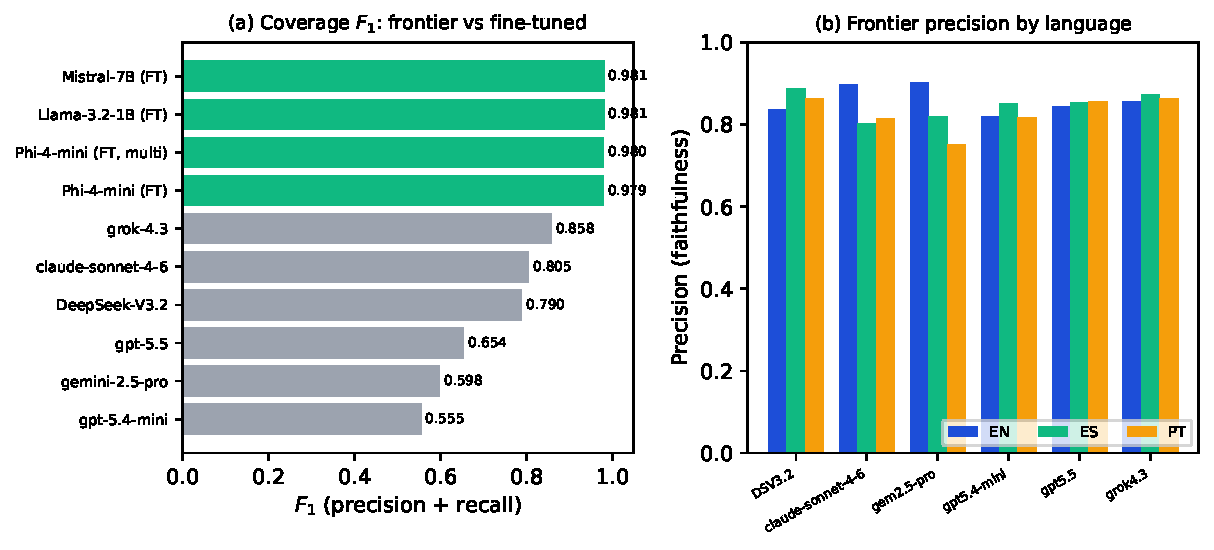
\includegraphics[width=0.92\textwidth]{fig_results.pdf}
\caption{(a) Precision (faithfulness) on the held-out 2025 test: a fine-tuned 3B model
(\,*\,) surpasses the frontier on precision while staying informative (cf.\
Table~\ref{tab:coverage}). (b) Precision across languages.}
\label{fig:results}
\end{figure*}

We study: \textbf{RQ1} -- does precision-only faithfulness reward abstention, and does
requiring coverage change which models look best?; \textbf{RQ2} -- does faithfulness vary
across languages?; \textbf{RQ3} -- can a fine-tuned small model match or exceed the
frontier? We evaluate the latest frontier models from four families zero-shot: OpenAI
gpt-5.5 and gpt-5.4-mini (Azure), xAI grok-4.3, Google gemini-2.5-pro (Vertex AI), and
DeepSeek-V3.2, each scored with the language-agnostic LLM claim extractor. Even these
models leave a non-trivial fraction of claims ungrounded and produce hard contradictions
(Table~\ref{tab:coverage}): fluent, expert-sounding narratives are not automatically
faithful.

\paragraph{Precision rewards abstention; coverage inverts the ranking (RQ1).}
Table~\ref{tab:coverage} reports precision (faithfulness), recall (coverage), and $F_1$
against the complete oracle. The most precise model, gemini-2.5-pro (precision
$\CovGeminiPrec{}$ in English), covers only $\CovGeminiRecall{}$ of the facts that
mattered -- it is the most faithful and the least informative, averaging under two claims
per instance. Conversely, more verbose models are slightly less precise but far more
complete. The consequence is decisive: ranking models by precision puts gemini-2.5-pro
\emph{first}, but ranking by $F_1$ puts it \emph{last} ($F_1=\CovGeminiFone{}$), with
\CovTopFoneModel{} -- mid-pack on precision -- now on top ($F_1=\CovTopFone{}$). A
precision-only faithfulness metric therefore does not just mis-score an output, it
\emph{reverses} the comparison between systems. This is the paper's central finding, and
it is measurable only because the oracle is complete.

\paragraph{Multilingual (RQ2).} Faithfulness is largely stable across EN/ES/PT for four of
the five models (Table~\ref{tab:coverage}); the apparent cross-lingual ``gap'' is
concentrated in gemini-2.5-pro, and it tracks the same terseness -- under one claim per
instance in ES/PT -- that drives its low coverage, rather than a general failure of
grounding to transfer. The drop persists under a cross-family extractor
(below), so it is not an extractor artifact. The practical reading is the opposite of the
naive one: across these models, \emph{how much} a model says (coverage) varies more, and
matters more, than the language it says it in.

\paragraph{Small fine-tuned model and verifier-guided method (RQ3).}
Table~\ref{tab:models} compares an open small model (Qwen2.5-3B
\citep{qwen2025}) zero-shot and after LoRA fine-tuning on grounded explanations, on a
common subset under the same LLM extractor. Read through the precision/coverage lens of
RQ1, the fine-tuned 3B model is the encouraging case: it attains the highest precision in
the table while \emph{also} staying substantive -- more claims per instance than
gemini-2.5-pro -- so, unlike gemini, its high faithfulness is not bought by abstention.
We read this as domain specialization on grounded supervision buying precision that scale
alone does not, without the terseness that would empty it out, echoing evidence that
small, specialized models are competitive in focused domains \citep{vectrayxnano2026}; the
silver template supervision is a caveat we discuss in Limitations. Separately,
verifier-guided self-correction (Section~\ref{sec:method}) applied to \MethodModel{}
raises precision from $\MethodFirst{}$ to $\MethodFinal{}$ (English regex verifier),
suggesting the structured verifier is a usable training-free signal.

\paragraph{Extractor robustness.} A concern with an LLM-scored metric is that the
extractor (gpt-5.x) shares a family with one evaluated system (gpt-5.5), which could
inflate its score. We re-score the \emph{same} generations with two independent
extractors. (i) A model-free, deterministic \emph{regex} extractor (English): it agrees
with the LLM extractor on the system ranking (Spearman $\ExtractorEnSpearman{}$) and at
the instance level (Pearson $\ExtractorEnPearson{}$, $N=\ExtractorEnN{}$). (ii) A
\emph{cross-family} LLM extractor (\XfamModel{}, no shared lineage with gpt-5.x), across
all three languages: agreement is near-perfect at the system level (Spearman
$\XfamSpearman{}$) and strong per instance (Pearson $\XfamPearson{}$, $N=\XfamN{}$),
higher than the metric's correlation with the independent LLM judge. The same-family
system, gpt-5.5, is not ranked top by its own family's extractor under either check. The
gemini-2.5-pro cross-lingual drop reproduces under the cross-family extractor, confirming
it is a property of the generations, not the extractor.

\IfFileExists{coverage_table.tex}{\begin{table*}[t]
\centering\small
\begin{tabular}{llcccc}
\toprule
Model & Lang & Prec. & Recall & F1 & Cl./inst. \\
\midrule
DeepSeek-V3.2$^{-71}$ & EN & 0.818 & 0.763 & 0.790 & 9.6 \\
DeepSeek-V3.2$^{-3}$ & ES & 0.841 & 0.719 & 0.776 & 9.3 \\
DeepSeek-V3.2$^{-3}$ & PT & 0.855 & 0.495 & 0.627 & 6.4 \\
gemini-2.5-pro & EN & 0.824 & 0.469 & 0.598 & 5.2 \\
gemini-2.5-pro & ES & 0.845 & 0.451 & 0.588 & 4.9 \\
gemini-2.5-pro$^{-1}$ & PT & 0.855 & 0.483 & 0.617 & 4.6 \\
gpt-5.4-mini & EN & 0.820 & 0.420 & 0.555 & 5.0 \\
gpt-5.4-mini & ES & 0.863 & 0.473 & 0.611 & 4.7 \\
gpt-5.4-mini & PT & 0.850 & 0.493 & 0.624 & 5.3 \\
gpt-5.5 & EN & 0.861 & 0.528 & 0.654 & 5.9 \\
gpt-5.5 & ES & 0.867 & 0.499 & 0.634 & 5.3 \\
gpt-5.5 & PT & 0.886 & 0.511 & 0.648 & 5.4 \\
grok-4.3$^{-71}$ & EN & 0.878 & 0.838 & 0.858 & 8.9 \\
grok-4.3$^{-3}$ & ES & 0.901 & 0.710 & 0.794 & 6.8 \\
grok-4.3$^{-3}$ & PT & 0.887 & 0.462 & 0.608 & 4.3 \\
claude-sonnet-4-6 & EN & 0.897 & 0.730 & 0.805 & 8.2 \\
claude-sonnet-4-6 & ES & 0.801 & 0.832 & 0.817 & 10.6 \\
claude-sonnet-4-6 & PT & 0.815 & 0.844 & 0.829 & 11.7 \\
\midrule
\multicolumn{6}{l}{\emph{Small models LoRA-fine-tuned on the complete oracle (this work)}}\\
\midrule
Llama-3.2-1B (FT) & EN & 0.994 & 0.968 & \textbf{0.981} & 5.6 \\
Phi-4-mini (FT) & EN & 0.994 & 0.965 & \textbf{0.979} & 5.6 \\
Mistral-7B (FT) & EN & 0.994 & 0.967 & \textbf{0.981} & 5.6 \\
Phi-4-mini (FT, multitask) & EN & 0.993 & 0.968 & \textbf{0.980} & 5.6 \\
\bottomrule
\end{tabular}
\caption{Precision (faithfulness) is gameable by abstention: against the \emph{complete} oracle we also measure recall (coverage of the facts that mattered). The most precise model is \emph{not} the most informative; requiring coverage ($F_1$) reorders the systems (e.g.\ in \CovLang{}, the most precise model, \CovFlipModel{}, ranks \CovFlipFRank{} by $F_1$). Only a complete structured oracle makes recall measurable. \textbf{Fine-tuning on the complete oracle closes the gap}: every FT model---even 1B---reaches $F_1 \approx 0.98$, beating every frontier system while remaining substantive. $^{-n}$: $n$ English instances dropped by platform content-filtering (same instances across AIServices models; not model behavior).}
\label{tab:coverage}
\end{table*}
}{}
\IfFileExists{weather_table.tex}{\begin{table*}[t]
\centering\small
\begin{tabular}{llcccc}
\toprule
Model & Lang & Prec. & Recall & F1 & Cl./inst. \\
\midrule
DeepSeek-V3.2 & EN & 0.865 & 0.843 & 0.854 & 5.5 \\
DeepSeek-V3.2 & ES & 0.910 & 0.653 & 0.761 & 4.2 \\
DeepSeek-V3.2 & PT & 0.854 & 0.413 & 0.557 & 2.8 \\
gemini-2.5-pro & EN & 0.912 & 0.250 & 0.393 & 1.3 \\
gemini-2.5-pro & ES & 0.836 & 0.215 & 0.342 & 1.1 \\
gemini-2.5-pro & PT & 0.868 & 0.208 & 0.336 & 1.0 \\
gpt-5.4-mini & EN & 0.944 & 0.462 & 0.620 & 2.9 \\
gpt-5.4-mini & ES & 0.916 & 0.442 & 0.596 & 2.8 \\
gpt-5.4-mini & PT & 0.953 & 0.460 & 0.621 & 2.9 \\
gpt-5.5 & EN & 0.936 & 0.470 & 0.626 & 3.0 \\
gpt-5.5 & ES & 0.932 & 0.458 & 0.615 & 2.9 \\
gpt-5.5 & PT & 0.946 & 0.457 & 0.616 & 2.9 \\
grok-4.3 & EN & 0.939 & 0.473 & 0.629 & 2.9 \\
grok-4.3 & ES & 0.948 & 0.460 & 0.620 & 2.9 \\
grok-4.3 & PT & 0.974 & 0.450 & 0.616 & 2.8 \\
\bottomrule
\end{tabular}
\caption{Second domain (weather, NOAA forecasts; complete record oracle). The abstention effect replicates outside F1: the same model that abstains there (gemini-2.5-pro) again states the fewest facts and has by far the lowest recall, so precision and $F_1$ disagree on the ranking. The effect is milder than in F1, as weather records have fewer facts to omit.}
\label{tab:weather}
\end{table*}
}{}
\IfFileExists{models_table.tex}{\begin{table}[t]
\centering\small
\resizebox{\columnwidth}{!}{%
\begin{tabular}{lccc}
\toprule
System (EN) & Faithf. & Halluc. & Claims/inst. \\
\midrule
DeepSeek-V3.2 (zero-shot) & 0.838 & 0.050 & 7.8 \\
gemini-2.5-pro (zero-shot) & 0.901 & 0.079 & 3.0 \\
gpt-5.4-mini (zero-shot) & 0.819 & 0.081 & 8.3 \\
gpt-5.5 (zero-shot) & 0.843 & 0.031 & 9.9 \\
grok-4.3 (zero-shot) & 0.855 & 0.022 & 8.6 \\
Qwen2.5-3B (zero-shot) & 0.831 & 0.101 & 7.0 \\
Qwen2.5-3B (fine-tuned) & 0.995 & 0.005 & 5.6 \\
\bottomrule
\end{tabular}}
\caption{Small open model (Qwen2.5-3B) before/after fine-tuning vs.\ frontier on the held-out 2025 test sample, English, same LLM-extractor metric. Faithfulness is read alongside coverage (claims per instance): the fine-tuned model is both more faithful and more concise. Fine-tuned only on \FOneFirstSeason{}--2024 (no test leakage).}
\label{tab:models}
\end{table}
}{}
\IfFileExists{extractor_agreement.tex}{% Auto-generated by experiments/extractor_agreement.py
\begin{table}[t]
\centering
\small
\begin{tabular}{lcc}
\toprule
Model & Regex (EN) & LLM (EN) \\
\midrule
DeepSeek-V3.2 & 0.735 & 0.838 \\
gemini-2.5-pro & 0.925 & 0.901 \\
gpt-5.4-mini & 0.742 & 0.819 \\
gpt-5.5 & 0.753 & 0.843 \\
grok-4.3 & 0.749 & 0.855 \\
\bottomrule
\end{tabular}
\caption{English faithfulness under the model-free regex extractor vs.\ the LLM extractor (gpt-5.x). The two extractors agree on the system-level ranking (Spearman $0.8$; same top model) and correlate at the instance level (Pearson $0.4984$, $N=564$), showing the English results are not an artifact of the LLM extractor's family. The regex extractor's ES/PT patterns are deliberately light, so it serves as an English-first cross-check.}
\label{tab:extractor}
\end{table}
}{}

\section{Generalization: A Second Oracle}\label{sec:weather}
The abstention problem is a claim about reference-free precision metrics in general, not
about F1. We replicate it in a second domain with a complete oracle: public-domain NOAA
weather forecasts, where each record (temperature, wind, precipitation chance, sky) is the
enumerable fact set a forecast should cover. We generate forecasts grounded in $150$
records per language with the same five models and score them with the same
precision/recall machinery (Table~\ref{tab:weather}). The effect reappears: the model that
abstains on F1, gemini-2.5-pro, again states the fewest facts ($\WxGeminiClaims{}$ claims
per instance) and has by far the lowest recall ($\WxGeminiRecall{}$ vs.\ $\WxOthersRecall{}$
for the others), so ranking by precision and by $F_1$ disagree ($F_1$ inversion present in
English). The effect is milder than in F1 -- a weather record has only a handful of facts,
so there is less to omit -- which is itself informative: the abstention penalty scales with
how much a faithful answer \emph{should} contain. That the same model abstains in two
unrelated domains suggests this is a property of the model and the precision-only metric,
not of any one dataset.

\section{Ethics and Licensing}\label{sec:ethics}
F1/FOM timing data carries usage restrictions; we release only code, derived
structured data, and annotations, not raw broadcast/telemetry feeds. The
benchmark concerns strategy explanation, not betting or outcome prediction.

\section{Limitations}
Our recall metric measures coverage of the facts our deterministic extractor derives;
these are high-precision but not exhaustive (event detection uses heuristics), so recall
is defined relative to this enumerable fact set rather than to every conceivable salient
detail -- the completeness we rely on is completeness \emph{of the derived oracle}. The
abstention finding is a property of reference-free precision metrics in general; we
demonstrate it in one domain, and replicating the precision/recall inversion in a second
complete-oracle domain (e.g.\ finance or weather data-to-text) is the natural next step.
The claim extractor can miss or over-segment claims, so absolute scores should be read
alongside the controlled-perturbation validation; we mitigate the concern that the
gpt-5.x extractor shares a family with gpt-5.5 with a model-free regex extractor and a
cross-family LLM extractor that agree closely with it (Section~\ref{sec:exp}), but a
human extractor/judge remains future work. Fine-tuning supervision is silver
(deterministic faithful templates), which risks rewarding template mimicry; stronger
supervision and out-of-template evaluation are future work. The model comparison uses a
stratified test sample for cost, covers EN/ES/PT, and the held-out split is a single
season (2022 omitted: timing data unavailable). Our quantitative comparison focuses on
the three core decision types (strategy, undercut, overcut); the defense and
race-summary types are released and exercised in the demo, with full model evaluation
left to future work.

\bibliography{refs}

\end{document}
